% stuff

\documentclass[prl,twocolumn,showpacs,superscriptaddress,preprintnumbers,floatfix]{revtex4-1}

% ******************************************************************************
% Imports

\usepackage{etex}                        %
\usepackage{ifpdf}                       %
\usepackage[final,pagebackref]{hyperref} %
\usepackage{graphicx}                    %
\usepackage{dcolumn}                     %
\usepackage{url}                         %
\usepackage{amsmath}                     %
\usepackage{amscd}                       %
\usepackage{amsfonts}                    %
\usepackage{amssymb}                     %
\usepackage{amsthm}                      %
\usepackage{bm}                          %
\usepackage{bbm}                         %
\usepackage{verbatim}                    %
\usepackage{stmaryrd}                    %
\usepackage{xcolor}                      %
\usepackage{setspace}                    %
\usepackage{xspace}                      % Let macros play nice with spaces
\usepackage{nicefrac}                    % Pretty fractions
\usepackage{cleveref}                    % Automatically label references
\usepackage{booktabs}                    % Nicer tables
\usepackage[caption=false]{subfig}       % Subfigures

% Various tikz related imports
\usepackage{tikz}
\usetikzlibrary{arrows}
\usetikzlibrary{automata}
\usetikzlibrary{calc}
\usetikzlibrary{decorations.pathreplacing}
\usetikzlibrary{external}
\usetikzlibrary{intersections}
\usetikzlibrary{patterns}
\usetikzlibrary{plotmarks}
\usetikzlibrary{positioning}
\usetikzlibrary{through}
%\tikzexternalize
\tikzsetexternalprefix{images/}
\tikzstyle{vaucanson}=[
  %node distance=1.25cm,
  node distance=3cm,
  bend angle=15,
  auto,
  % For some reason, the loop direction cannot be overwritten if we set the
  % style for "every loop" to be "->".  Curiously, this doesn't seem to be
  % an issue for "every edge".
  every loop/.style={},
  every edge/.style={->,draw=black,line width=1.2,>=latex,shorten <=1pt, shorten >=1pt},
  every state/.style={draw=black,line width=2,font=\large},
  loop right/.style={right,out=22,in=-22,loop},
  loop above/.style={above,out=112,in=68,loop},
  loop left/.style={left,out=202,in=158,loop},
  loop below/.style={below,out=292,in=248,loop},
  loop above right/.style={right,out=67,in=23,loop},
  loop above left/.style={left,out=157,in=113,loop},
  loop below left/.style={left,out=247,in=203,loop},
  loop below right/.style={right,out=337,in=293,loop},
  binode/.style={minimum size=1cm,inner sep=0pt},
]

\tikzset{
  mystate/.style={circle,draw,fill=black}
}

%%% Command for bicausal nodes. This only supports relative positioning.
%%% Use as: \binode[state][red,blue] (AC) [left=of someNode] {$\A:\:C$};
\makeatletter
\newcommand{\binode}[1][state]{%
  \@ifnextchar[{\binode@i[{#1}]}{\binode@i[{#1}][{yellow},{gray!70}]}%
}
\def\binode@i[#1][#2,#3]{%
  \@ifnextchar({\binode@ii[{#1}][{#2},{#3}]}{\binode@ii[{#1}][{#2},{#3}]({})}%
}
\def\binode@ii[#1][#2,#3](#4){%
  \@ifnextchar[{\binode@iii[{#1}][{#2},{#3}]({#4})}{\binode@iii[{#1}][{#2},{#3}]({#4})[{}]}%
}
\def\binode@iii[#1][#2,#3](#4)[#5]#6{%

  \node[#1,binode] (#4) [#5] {#6};
  \node[yshift=-10pt] (#4SS) at (#4.270) {};
  \node[xshift=-10pt] (#4WW) at (#4.180) {};
  \node[xshift=-10pt] (#4NN) at (#4.180) {};
  \node[xshift=-10pt,yshift=10pt] (#4NW) at (#4.135) {};
  % forward shading
  \begin{scope}
    \path[clip] (#4.255) -- +(-.8cm,0cm) -- +(-.8cm,1cm) -- (#4.75) -- cycle;
    \node[#1,fill=#2,binode] (#4f) [#5] {#6};
  \end{scope}
  % reverse shading
  \begin{scope}
    \path[clip] (#4.75) -- +(.8cm,0cm) -- +(.8cm,-1cm) -- (#4.255) -- cycle;
%    ++(0cm,-.2cm) -- ++(.8cm,0cm)  -- ++(0cm,1cm) -- (#4.75) -- cycle;
    \node[#1,fill=#3,binode] (#4r) [#5] {#6};
  \end{scope}
  \node {} % semicolon purposefully omitted. this is a dummy call
}
\makeatother

\providecommand{\Symbol}[1]{\textcolor{blue}{#1}}
\providecommand{\Edge}[2]{\Symbol{#1} : #2}

\definecolor{FCSA}{RGB}{141,211,199}
\definecolor{FCSB}{RGB}{255,255,179}
\definecolor{RCSC}{RGB}{185,138,196}
\definecolor{RCSD}{RGB}{231,143,111}
\definecolor{RCSE}{RGB}{128,177,211}




\usepackage{pgfplots}
\pgfplotsset{compat=newest}

% Useful code stolen from http://tex.stackexchange.com/a/71596/66712
\tikzset{
  anticlockwise arc centered at/.style={
    to path={
      let \p1=(\tikztostart), \p2=(\tikztotarget), \p3=(#1) in
      \pgfextra{
        \pgfmathsetmacro{\anglestart}{atan2(\x1-\x3,\y1-\y3)}
        \pgfmathsetmacro{\angletarget}{atan2(\x2-\x3,\y2-\y3)}
        \pgfmathsetmacro{\angletarget}%
        {\angletarget < \anglestart ? \angletarget+360 : \angletarget}
        \pgfmathsetmacro{\radius}{veclen(\x1-\x3,\y1-\y3)}
      }
      arc(\anglestart:\angletarget:\radius pt) -- (\tikztotarget)
    },
  },
  clockwise arc centered at/.style={
    to path={
      let \p1=(\tikztostart), \p2=(\tikztotarget), \p3=(#1) in
      \pgfextra{
        \pgfmathsetmacro{\anglestart}{atan2(\x1-\x3,\y1-\y3)}
        \pgfmathsetmacro{\angletarget}{atan2(\x2-\x3,\y2-\y3)}
        \pgfmathsetmacro{\angletarget}%
        {\angletarget > \anglestart ? \angletarget - 360 : \angletarget}
        \pgfmathsetmacro{\radius}{veclen(\x1-\x3,\y1-\y3)}
      }
      arc(\anglestart:\angletarget:\radius pt) -- (\tikztotarget)
    },
  },
}

% Used for code samples
\usepackage{listings}
\lstdefinestyle{mypython}{
language=Python,                        % Code langugage
basicstyle=\small\ttfamily,             % Code font, Examples: \footnotesize, \ttfamily
keywordstyle=\color{green!50!black},    % Keywords font ('*' = uppercase)
commentstyle=\color{gray},              % Comments font
numbers=left,                           % Line nums position
numberstyle=\tiny,                      % Line-numbers fonts
stepnumber=1,                           % Step between two line-numbers
numbersep=5pt,                          % How far are line-numbers from code
backgroundcolor=\color{gray!10},        % Choose background color
frame=none,                             % A frame around the code
tabsize=2,                              % Default tab size
captionpos=b,                           % Caption-position = bottom
breaklines=true,                        % Automatic line breaking?
breakatwhitespace=false,                % Automatic breaks only at whitespace?
showspaces=false,                       % Dont make spaces visible
showtabs=false,                         % Dont make tabls visible
morekeywords={as},                      % Additional keywords
}



\DeclareMathOperator*{\argmin}{argmin}
\DeclareMathOperator*{\argmax}{argmax}

% Abbreviations from CMPPSS:

\newcommand{\eM}     {\mbox{$\epsilon$-machine}}
\newcommand{\eMs}    {\mbox{$\epsilon$-machines}}
\newcommand{\EM}     {\mbox{$\epsilon$-Machine}}
\newcommand{\EMs}    {\mbox{$\epsilon$-Machines}}
\newcommand{\eT}     {\mbox{$\epsilon$-transducer}}
\newcommand{\eTs}    {\mbox{$\epsilon$-transducers}}
\newcommand{\ET}     {\mbox{$\epsilon$-Transducer}}
\newcommand{\ETs}    {\mbox{$\epsilon$-Transducers}}

% cryptic
\newcommand{\order}[1]{order\protect\nobreakdash-$#1$}
\newcommand{\Order}[1]{Order\protect\nobreakdash-$#1$}
\newcommand{\cryptic}[1]{$#1$\protect\nobreakdash-cryptic}
\newcommand{\Cryptic}[1]{$#1$\protect\nobreakdash-Cryptic}
\newcommand{\crypticity}[1]{$#1$\protect\nobreakdash-crypticity}
\newcommand{\Crypticity}[1]{$#1$\protect\nobreakdash-Crypticity}

% Processes and sequences

\newcommand{\Process}{\mathcal{P}}

\newcommand{\ProbMach}{\Prob_{\mathrm{M}}}
\newcommand{\Lmax}   { {L_{\mathrm{max}}}}
\newcommand{\MeasAlphabet}      {\mathcal{A}}
% Original symbol
%\newcommand{\MeasSymbol}   { {S} }
%\newcommand{\meassymbol}   { {s} }
% New symbol
\newcommand{\MeasSymbol}   { {X} }
\newcommand{\meassymbol}   { {x} }
\newcommand{\BiInfinity}        { \smash{\overleftrightarrow {\MeasSymbol}} }
\newcommand{\biinfinity}        { \smash{\overleftrightarrow {\meassymbol}} }
\newcommand{\Past}      { \smash{\overleftarrow {\MeasSymbol}} }
\newcommand{\past}      { \smash{\overleftarrow {\meassymbol}} }
\newcommand{\pastprime} { {\past}^{\prime}}
\newcommand{\Future}    { \smash{\overrightarrow{\MeasSymbol}} }
\newcommand{\future}    { \smash{\overrightarrow{\meassymbol}} }
\newcommand{\futureprime}       { \smash{\future^{\prime}} }
\newcommand{\PastPrime}     { \smash{\Past^{\prime}} }
\newcommand{\FuturePrime}       { \smash{\overrightarrow{\meassymbol}^\prime} }
\newcommand{\PastDblPrime}      { \smash{\overleftarrow{\meassymbol}^{\prime\prime}} }
\newcommand{\FutureDblPrime}{ \smash{\overrightarrow{\meassymbol}^{\prime\prime}} }
\newcommand{\pastL}     { \smash{\overleftarrow {\meassymbol}{}^L} }
\newcommand{\PastL}     { \smash{\overleftarrow {\MeasSymbol}{}^L} }
\newcommand{\PastLt}      { \smash{\overleftarrow {\MeasSymbol}_t^L} }
\newcommand{\PastLLessOne}{ \smash{\overleftarrow {\MeasSymbol}^{L-1}} }
\newcommand{\futureL}     { \smash{\overrightarrow{\meassymbol}{}^L} }
\newcommand{\FutureL}     { \smash{\overrightarrow{\MeasSymbol}{}^L} }
\newcommand{\FutureLt}    { \smash{\overrightarrow{\MeasSymbol}_t^L} }
\newcommand{\FutureLLessOne}{ \smash{\overrightarrow{\MeasSymbol}^{L-1}} }
\newcommand{\pastLprime}        { \smash{\overleftarrow {\meassymbol}^{L^\prime}} }
\newcommand{\futureLprime}      { \smash{\overrightarrow{\meassymbol}^{L^\prime}} }
\newcommand{\AllPasts}      { \smash{\overleftarrow{ {\rm {\bf \MeasSymbol}} } } }
\newcommand{\AllFutures}        { \smash{\overrightarrow{ {\rm {\bf \MeasSymbol}} } } }
\newcommand{\FutureSet} { \smash{\overrightarrow{\bf \MeasSymbol}} }

% Causal states and epsilon-machines
\newcommand{\CausalState}       { \mathcal{S} }
\newcommand{\CausalStatePrime}  { {\CausalState}^{\prime}}
\newcommand{\causalstate}       { \sigma }
\newcommand{\CausalStateSet}    { \boldsymbol{\CausalState} }
\newcommand{\AlternateState}    { \mathcal{R} }
\newcommand{\AlternateStatePrime}       { {\cal R}^{\prime} }
\newcommand{\alternatestate}    { \rho }
\newcommand{\alternatestateprime}       { {\rho^{\prime}} }
\newcommand{\AlternateStateSet} { \boldsymbol{\AlternateState} }
\newcommand{\PrescientState}    { \widehat{\AlternateState} }
\newcommand{\prescientstate}    { \widehat{\alternatestate} }
\newcommand{\PrescientStateSet} { \boldsymbol{\PrescientState}}
\newcommand{\CausalEquivalence} { {\sim}_{\epsilon} }
\newcommand{\CausalEquivalenceNot}      { {\not \sim}_{\epsilon}}

\newcommand{\NonCausalEquivalence}      { {\sim}_{\eta} }
\newcommand{\NextObservable}    { {\smash{\overrightarrow {\MeasSymbol}}^1} }
\newcommand{\LastObservable}    { {\smash{\overleftarrow {\MeasSymbol}}^1} }
%\newcommand{\Prob}             { {\rm P}}
\newcommand{\Prob}      {\Pr} % use standard command
\newcommand{\ProbAnd}   { {,\;} }
\newcommand{\LLimit}    { {L \rightarrow \infty}}
\newcommand{\Cmu}               {C_\mu}
\newcommand{\hmu}               {h_\mu}
\newcommand{\EE}                {{\bf E}}
\newcommand{\TI}                {{\bf T}}
\newcommand{\SI}        {{\bf S}}
\newcommand{\Measurable}{{\bf \mu}}

% Process Crypticity
\newcommand{\PC}                {\chi}

% Causal Irreversibility
\newcommand{\CI}                {\Xi}
\newcommand{\ReverseMap}        {r}
\newcommand{\ForwardMap}        {f}

% Abbreviations from IB:
% None that aren't already in CMPPSS

% Abbreviations from Extensive Estimation:
\newcommand{\EstCausalState}    {\widehat{\CausalState}}
\newcommand{\estcausalstate}    {\widehat{\causalstate}}
\newcommand{\EstCausalStateSet} {\boldsymbol{\EstCausalState}}
\newcommand{\EstCausalFunc}     {\widehat{\epsilon}}
\newcommand{\EstCmu}            {\widehat{\Cmu}}
\newcommand{\PastLOne}  {{\Past}^{L+1}}
\newcommand{\pastLOne}  {{\past}^{L+1}}

% Abbreviations from $\epsilon$-Transducers:
\newcommand{\InAlphabet}        { \mathcal{A}}
\newcommand{\insymbol}          { a}
\newcommand{\OutAlphabet}       { \mathcal{B}}
\newcommand{\outsymbol}         { b}
\newcommand{\InputSimple}       { X}
\newcommand{\inputsimple}       { x}
\newcommand{\BottleneckVar}     {\tilde{\InputSimple}}
\newcommand{\bottleneckvar}     {\tilde{\inputsimple}}
\newcommand{\InputSpace}        { \mathbf{\InputSimple}}
\newcommand{\InputBi}   { \overleftrightarrow {\InputSimple} }
\newcommand{\inputbi}   { \overleftrightarrow {\inputsimple} }
\newcommand{\InputPast} { \overleftarrow {\InputSimple} }
\newcommand{\inputpast} { \overleftarrow {\inputsimple} }
\newcommand{\InputFuture}       { \overrightarrow {\InputSimple} }
\newcommand{\inputfuture}       { \overrightarrow {\inputsimple} }
\newcommand{\NextInput} { {{\InputFuture}^{1}}}
\newcommand{\NextOutput}        { {\OutputFuture}^{1}}
\newcommand{\OutputSimple}      { Y}
\newcommand{\outputsimple}      { y}
\newcommand{\OutputSpace}       { \mathbf{\OutputSimple}}
\newcommand{\OutputBi}  { \overleftrightarrow{\OutputSimple} }
\newcommand{\outputbi}  { \overleftrightarrow{\outputsimple} }
\newcommand{\OutputPast}        { \overleftarrow{\OutputSimple} }
\newcommand{\outputpast}        { \overleftarrow{\outputsimple} }
\newcommand{\OutputFuture}      { \overrightarrow{\OutputSimple} }
\newcommand{\outputfuture}      { \overrightarrow{\outputsimple} }
\newcommand{\OutputL}   { {\OutputFuture}^L}
\newcommand{\outputL}   { {\outputfuture}^L}
\newcommand{\InputLLessOne}     { {\InputFuture}^{L-1}}
\newcommand{\inputLlessone}     { {\inputufutre}^{L-1}}
\newcommand{\OutputPastLLessOne}        {{\OutputPast}^{L-1}_{-1}}
\newcommand{\outputpastLlessone}        {{\outputpast}^{L-1}}
\newcommand{\OutputPastLessOne} {{\OutputPast}_{-1}}
\newcommand{\outputpastlessone} {{\outputpast}_{-1}}
\newcommand{\OutputPastL}       {{\OutputPast}^{L}}
\newcommand{\OutputLPlusOne}    { {\OutputFuture}^{L+1}}
\newcommand{\outputLplusone}    { {\outputfutre}^{L+1}}
\newcommand{\InputPastL}        {{\InputPast}^{L}}
\newcommand{\inputpastL}        {{\inputpast}^{L}}
\newcommand{\JointPast} {{(\InputPast,\OutputPast)}}
\newcommand{\jointpast} {{(\inputpast,\outputpast)}}
\newcommand{\jointpastone}      {{(\inputpast_1,\outputpast_1)}}
\newcommand{\jointpasttwo}      {{(\inputpast_2,\outputpast_2)}}
\newcommand{\jointpastprime} {{({\inputpast}^{\prime},{\outputpast}^{\prime})}}
\newcommand{\NextJoint} {{(\NextInput,\NextOutput)}}
\newcommand{\nextjoint} {{(\insymbol,\outsymbol)}}
\newcommand{\AllInputPasts}     { { \overleftarrow {\rm \InputSpace}}}
\newcommand{\AllOutputPasts}    { {\overleftarrow {\rm \OutputSpace}}}
\newcommand{\DetCausalState}    { {{\cal S}_D }}
\newcommand{\detcausalstate}    { {{\sigma}_D} }
\newcommand{\DetCausalStateSet} { \boldsymbol{{\CausalState}_D}}
\newcommand{\DetCausalEquivalence}      { {\sim}_{{\epsilon}_{D}}}
\newcommand{\PrescientEquivalence}      { {\sim}_{\widehat{\eta}}}
\newcommand{\FeedbackCausalState}       { \mathcal{F}}
\newcommand{\feedbackcausalstate}       { \phi}
\newcommand{\FeedbackCausalStateSet}    { \mathbf{\FeedbackCausalState}}
\newcommand{\JointCausalState}          { \mathcal{J}}
\newcommand{\JointCausalStateSet}       { \mathbf{\JointCausalState}}
\newcommand{\UtilityFunctional} { {\mathcal{L}}}
\newcommand{\NatureState}       { {\Omega}}
\newcommand{\naturestate}       { {\omega}}
\newcommand{\NatureStateSpace}  { {\mathbf{\NatureState}}}
\newcommand{\AnAction}  { {A}}
\newcommand{\anaction}  { {a}}
\newcommand{\ActionSpace}       { {\mathbf{\AnAction}}}

% Abbreviations from RURO:
\newcommand{\InfoGain}[2] { \mathcal{D} \left( {#1} || {#2} \right) }

% Abbreviations from Upper Bound:
\newcommand{\lcm}       {{\rm lcm}}
% Double-check that this isn't in the math set already!

% Abbreviations from Emergence in Space
\newcommand{\ProcessAlphabet}   {\MeasAlphabet}
\newcommand{\ProbEst}                   { {\widehat{\Prob}_N}}
\newcommand{\STRegion}                  { {\mathrm K}}
\newcommand{\STRegionVariable}          { K}
\newcommand{\stregionvariable}          { k}
\newcommand{\GlobalPast}                { \overleftarrow{G}}
\newcommand{\globalpast}                { \overleftarrow{g}}
\newcommand{\GlobalFuture}              { \overrightarrow{G}}
\newcommand{\globalfuture}              { \overrightarrow{g}}
\newcommand{\GlobalState}               { \mathcal{G}}
\newcommand{\globalstate}               { \gamma}
\newcommand{\GlobalStateSet}            { {\mathbf \GlobalState}}
\newcommand{\LocalPast}                 { \overleftarrow{L}}
\newcommand{\localpast}                 { \overleftarrow{l}}
\newcommand{\AllLocalPasts}             { \mathbf{\LocalPast}}
\newcommand{\LocalPastRegion}           { \overleftarrow{\mathrm L}}
\newcommand{\LocalFuture}               { \overrightarrow{L}}
\newcommand{\localfuture}               { \overrightarrow{l}}
\newcommand{\LocalFutureRegion}         { \overrightarrow{\mathrm L}}
\newcommand{\LocalState}                { \mathcal{L}}
\newcommand{\localstate}                { \lambda}
\newcommand{\LocalStateSet}             { {\mathbf \LocalState}}
\newcommand{\PatchPast}                 { \overleftarrow{P}}
\newcommand{\patchpast}                 { \overleftarrow{p}}
\newcommand{\PatchPastRegion}           { \overleftarrow{\mathrm P}}
\newcommand{\PatchFuture}               { \overrightarrow{P}}
\newcommand{\patchfuture}               { \overrightarrow{p}}
\newcommand{\PatchFutureRegion}         { \overrightarrow{\mathrm P}}
\newcommand{\PatchState}                { \mathcal{P}}
\newcommand{\patchstate}                { \pi}
\newcommand{\PatchStateSet}             { {\mathbf \PatchState}}
\newcommand{\LocalStatesInPatch}        {\vec{\LocalState}}
\newcommand{\localstatesinpatch}        {\vec{\localstate}}
\newcommand{\PointInstantX}             { {\mathbf x}}
% Galles's original LaTeX for the cond. indep. symbol follows:
\newcommand{\compos}{\mbox{$~\underline{~\parallel~}~$}}
\newcommand{\ncompos}{\not\hspace{-.15in}\compos}
\newcommand{\indep}                     { \rotatebox{90}{$\models$}}
\newcommand{\nindep}    {\not\hspace{-.05in}\indep}
\newcommand{\LocalEE}   {{\EE}^{loc}}
\newcommand{\EEDensity} {\overline{\LocalEE}}
\newcommand{\LocalCmu}  {{\Cmu}^{loc}}
\newcommand{\CmuDensity}        {\overline{\LocalCmu}}

%%%%%%%%%%% added by sasa
\newcommand{\FinPast}[1]        { \overleftarrow {\MeasSymbol} \stackrel{{#1}}{}}
\newcommand{\finpast}[1]        { \overleftarrow {\meassymbol}  \stackrel{{#1}}{}}
\newcommand{\FinFuture}[1]              { \overrightarrow{\MeasSymbol} \stackrel{{#1}}{}}
\newcommand{\finfuture}[1]              { \overrightarrow{\meassymbol} \stackrel{{#1}}{}}

\newcommand{\Partition} { \AlternateState }
\newcommand{\partitionstate}    { \alternatestate }
\newcommand{\PartitionSet}      { \AlternateStateSet }
\newcommand{\Fdet}   { F_{\rm det} }

\newcommand{\Dkl}[2] { D_{\rm KL} \left( {#1} || {#2} \right) }

\newcommand{\Period}    {p}

% To take into account time direction
\newcommand{\forward}{+}
\newcommand{\reverse}{-}
%\newcommand{\forwardreverse}{\:\!\diamond} % \pm
\newcommand{\forwardreverse}{\pm} % \pm
\newcommand{\FutureProcess}     { {\Process}^{\forward} }
\newcommand{\PastProcess}       { {\Process}^{\reverse} }
\newcommand{\FutureCausalState} { {\CausalState}^{\forward} }
\newcommand{\futurecausalstate} { \sigma^{\forward} }
\newcommand{\altfuturecausalstate}      { \sigma^{\forward\prime} }
\newcommand{\PastCausalState}   { {\CausalState}^{\reverse} }
\newcommand{\pastcausalstate}   { \sigma^{\reverse} }
\newcommand{\BiCausalState}             { {\CausalState}^{\forwardreverse} }
\newcommand{\bicausalstate}             { {\sigma}^{\forwardreverse} }
\newcommand{\FutureCausalStateSet}      { {\CausalStateSet}^{\forward} }
\newcommand{\PastCausalStateSet}        { {\CausalStateSet}^{\reverse} }
\newcommand{\BiCausalStateSet}  { {\CausalStateSet}^{\forwardreverse} }
\newcommand{\eMachine}  { M }
\newcommand{\FutureEM}  { {\eMachine}^{\forward} }
\newcommand{\PastEM}    { {\eMachine}^{\reverse} }
\newcommand{\BiEM}              { {\eMachine}^{\forwardreverse} }
\newcommand{\BiEquiv}   { {\sim}^{\forwardreverse} }
\newcommand{\Futurehmu} { h_\mu^{\forward} }
\newcommand{\Pasthmu}   { h_\mu^{\reverse} }
\newcommand{\FutureCmu} { C_\mu^{\forward} }
\newcommand{\PastCmu}   { C_\mu^{\reverse} }
\newcommand{\BiCmu}             { C_\mu^{\forwardreverse} }
\newcommand{\FutureEps} { \epsilon^{\forward} }
\newcommand{\PastEps}   { \epsilon^{\reverse} }
\newcommand{\BiEps}     { \epsilon^{\forwardreverse} }
\newcommand{\FutureSim} { \sim^{\forward} }
\newcommand{\PastSim}   { \sim^{\reverse} }
\newcommand{\FuturePC}  {\PC^{\forward}}
\newcommand{\PastPC}            {\PC^{\reverse}}
\newcommand{\BiPC}      {\PC^{\forwardreverse}}

% Used arrows for awhile, more or less confusing?
%\newcommand{\FutureCausalState}        { \overrightarrow{\CausalState} }
%\newcommand{\PastCausalState}  { \overleftarrow{\CausalState} }
%\newcommand{\eMachine} { M }
%\newcommand{\FutureEM} { \overrightarrow{\eMachine} }
%\newcommand{\PastEM}   { \overleftarrow{\eMachine} }
%\newcommand{\FutureCmu}        { \overrightarrow{\Cmu} }
%\newcommand{\PastCmu}  { \overleftarrow{\Cmu} }

%% time-reversing and mixed state presentation operators
\newcommand{\TR}{\mathcal{T}}
\newcommand{\MSP}{\mathcal{U}}
\newcommand{\one}{\mathbf{1}}

%% added for RURO2
%% Note that it will always be typesett in math mode.
%% Example usage:
%%    The 3-block entropy is \BE[t]{3}.
%%    The 3-block-state entropy from $t=0$ is $\BSE{3}$.
%%
%% The optional argument specifies the start time, defaulting to t=0.
%% The mandatory argument specifies the length of the block (not the stop time).
\newcommand{\lastindex}[2]{
  \edef\tempa{0}
  \edef\tempb{#2}
  \ifx\tempa\tempb
    % if the length is 0, then the final time equals the start time
    \edef\tempc{#1}
  \else
    % if the start time is different from zero, then we show the sum
    \edef\tempa{0}
    \edef\tempb{#1}
    \ifx\tempa\tempb
      \edef\tempc{#2}
    \else
      \edef\tempc{#1+#2}
    \fi
  \fi
  \tempc
}
\newcommand{\BE}[2][0]{
  \ensuremath{H[\MeasSymbol_{#1}^{#2}]}
}
\newcommand{\BSE}[2][0]{
  \ensuremath{H[\MeasSymbol_{#1}^{#2},\CausalState_{\lastindex{#1}{#2}}]}%
}
\newcommand{\SBE}[2][0]{
  \ensuremath{H[\CausalState_{#1},\MeasSymbol_{#1}^{#2}]}
}
\newcommand{\SBSE}[2][0]{
  \ensuremath{H[\CausalState_{#1},\MeasSymbol_{#1}^{#2},
                \CausalState_{\lastindex{#1}{#2}}]}
}
\newcommand{\AltSBE}[2][0]{
  \ensuremath{H[\AlternateState_{#1},\MeasSymbol_{#1}^{#2}]}
}
\newcommand{\AltBSE}[2][0]{
  \ensuremath{H[\MeasSymbol_{#1}^{#2},\AlternateState_{\lastindex{#1}{#2}}]}
}
\newcommand{\AltSBSE}[2][0]{
  \ensuremath{H[\AlternateState_{#1},\MeasSymbol_{#1}^{#2},
                \AlternateState_{\lastindex{#1}{#2}}]}
}

\newcommand{\GI}{\varphi}
\newcommand{\OI}{\zeta}
% cryptic, gauge, oracular, Markov, and synchronization
\newcommand{\COrder}{k_{\PC}}
\newcommand{\GOrder}{k_{\GI}}
\newcommand{\OOrder}{k_{\OI}}
\newcommand{\MOrder}{R}
\newcommand{\SOrder}{k_{\SI}}

%%% anatomy of a bit related quantities:

\newcommand{\metric}[1] {\ensuremath{#1_\mu}\xspace}

\newcommand{\rhomu}{\metric{\rho}}
\newcommand{\rmu}{\metric{r}}
\newcommand{\bmu}{\metric{b}}
\newcommand{\qmu}{\metric{q}}
\newcommand{\wmu}{\metric{w}}
\newcommand{\imu}{\metric{i}}
\newcommand{\sigmamu}{\metric{\sigma}}
\newcommand{\EER}{\EE_R}
\newcommand{\EEB}{\EE_B}
\newcommand{\EEQ}{\EE_Q}
\newcommand{\EEW}{\EE_W}
\newcommand{\I}{\mathbf{I}}

%% Added to standardize the order of causal states
%% Example usage:
%%    $\BiCmu = H[\CSjoint] = H[\CSjoint[,]]$
%%    $\EE = I[\CSjoint[:]] = I[\CSjoint[;]]$
\newcommand{\CSjoint}[1][,]{
   \edef\tempa{:}
   \edef\tempb{#1}
   \ifx\tempa\tempb
      % arg1 was a colon, insert a small negative space
      \ensuremath{\FutureCausalState\!#1\PastCausalState}
   \else
      % arg1 was not a colon, usually a comma or semicolon
      \ensuremath{\FutureCausalState#1\PastCausalState}
   \fi
}
\newcommand{\CSjointKL}[3][,]{
   \edef\tempa{:}
   \edef\tempb{#1}
   \ifx\tempa\tempb
      % arg1 was a colon, insert a small negative space
      \ensuremath{\FutureCausalState_{#2}\!#1\PastCausalState_{#3}}
   \else
      % arg1 was not a colon, usually a comma or semicolon
      \ensuremath{\FutureCausalState_{#2}#1\PastCausalState_{#3}}
   \fi
}


%% (cje)
%% Provide a command \ifpm which is true when \pm
%% is meant to be understood as "+ or -", opposed
%% to "bidirectional". This differs from the usage
%% in TBA.  Essentially, if \forwardreverse is defined
%% as something different, perhaps a \diamond, then
%% we are free to interpret \pm as "+ or -".
\newif\ifpm
\edef\tempa{\forwardreverse}
\edef\tempb{\pm}
\ifx\tempa\tempb
   \pmfalse
\else
   \pmtrue
\fi

%% Macros for krorder
\newcommand{\MeasSymbols}[2] {\ensuremath{\MeasSymbol_{#1:#2}}\xspace}
\newcommand{\Lsync} {\mathcal{L}_{\mathrm{sync}}}
\renewcommand{\Past}{\MeasSymbols{}{0}}
\newcommand{\Present}{\ensuremath{\MeasSymbol_0}}
\renewcommand{\Future}{\MeasSymbols{1}{}}

%% infotheory macros
\newcommand{\op}  [2]   {\ensuremath{\operatorname{#1}\left[#2\right]}\xspace}

\renewcommand{\H} [1]   {\op{H}{#1}}
\renewcommand{\I} [1]   {\op{I}{#1}}
\newcommand{\T}   [1]   {\op{T}{#1}}
\newcommand{\R}   [1]   {\op{R}{#1}}
\newcommand{\B}   [1]   {\op{B}{#1}}
\newcommand{\K}   [1]   {\op{K}{#1}}

\newcommand{\meet}      {\curlywedge}
\newcommand{\join}      {\curlyvee}
\newcommand{\iless}     {\preceq}
\newcommand{\imore}     {\succeq}
\newcommand{\ieq}       {\cong}
\newcommand{\mss}       {\downrightarrow}


\newcommand{\half}{\ensuremath{\nicefrac{1}{2}}}


%\listfiles

\parskip 0pt

\newcommand{\alert}[1]{\textbf{\textcolor{red}{#1}}}


\theoremstyle{plain}    \newtheorem{Lem}{Lemma}
\theoremstyle{plain}    \newtheorem*{ProLem}{Proof}
\theoremstyle{plain}    \newtheorem{Cor}{Corollary}
\theoremstyle{plain}    \newtheorem*{ProCor}{Proof}
\theoremstyle{plain}    \newtheorem{The}{Theorem}
\theoremstyle{plain}    \newtheorem*{ProThe}{Proof}
\theoremstyle{plain}    \newtheorem{Prop}{Proposition}
\theoremstyle{plain}    \newtheorem*{ProProp}{Proof}
\theoremstyle{plain}    \newtheorem*{Conj}{Conjecture}
\theoremstyle{plain}    \newtheorem*{Rem}{Remark}
\theoremstyle{plain}    \newtheorem{Def}{Definition}
\theoremstyle{plain}    \newtheorem*{Not}{Notation}

% ******************************************************************************
% Set up pdf stuff

\newcommand{\arxiv}[1]{\href{http://arxiv.org/abs/#1}{\texttt{arXiv}:#1}}
 % SFI working papers do not have friendly URLs.
\newcommand{\sfiwp}[1]{Santa Fe Institute Working Paper #1}

\begin{document}

\def\ourTitle{Further Anatomy of a Bit}

\title{\ourTitle}

\def\ourAbstract{%
  In our prior work, we decomposed the joint distribution $\H{\Past, \Present,
  \Future} = \H{\FCS_0, \Present, \RCS_1}$, exposing new insight in to how
  complex processes store, process, and generate information. Here, we
  incorporate the generating dynamic in to this picture by decomposing the
  distribution \H{\FCS_0, \Present, \FCS_1, \RCS_1} revealing an even more
  detailed picture of the inner workings of a process.
}

\def\ourKeywords{%
 stochastic process, hidden Markov model,
  \texorpdfstring{\eM}{epsilon-machine}, causal states, mutual information.
}

\hypersetup{
  pdfauthor={Ryan G. James},
  pdftitle={\ourTitle},
  pdfsubject={\ourAbstract},
  pdfkeywords={\ourKeywords},
  pdfproducer={},
  pdfcreator={}
}

\author{Ryan G. James}
\email{rgjames@ucdavis.edu}
\affiliation{Complexity Sciences Center and Physics Department,
University of California at Davis, One Shields Avenue, Davis, CA 95616}

% \author{John Mahoney}
% \email{jmahony@ucdavis.edu}
% \affiliation{Complexity Sciences Center and Physics Department,
% University of California at Davis, One Shields Avenue, Davis, CA 95616}

\author{James P. Crutchfield}
\email{chaos@ucdavis.edu}
\affiliation{Complexity Sciences Center and Physics Department,
University of California at Davis, One Shields Avenue, Davis, CA 95616}
\affiliation{Santa Fe Institute, 1399 Hyde Park Road, Santa Fe, NM 87501}

\date{\today}
\bibliographystyle{unsrt}


% ******************************************************************************
% TikZ graphics setup

\colorlet {past_color}    {red}
\colorlet {pres_color}    {blue}
\colorlet {futu_color}    {black!30!green}

\colorlet {temp_color_1}  {red!50!blue}
\colorlet {temp_color_2}  {red!50!green}
\colorlet {temp_color_3}  {blue!50!green}

\colorlet {hmu_color}     {blue!67!green}
\colorlet {rhomu_color}   {temp_color_1!80!blue}
\colorlet {rmu_color}     {blue}
\colorlet {bmu_1_color}   {temp_color_1}
\colorlet {bmu_2_color}   {temp_color_3}
\colorlet {qmu_color}     {temp_color_1!67!green}
\colorlet {wmu_color}     {temp_color_2!57!blue}
\colorlet {sigmamu_color} {temp_color_2}

\def \idiagramsetup {
  \def \radius {1.5}
  \def \delt {2}
  \def \diff {0.04}

  \coordinate (A) at (0, 0);
  \coordinate (B) at (240:\delt);
  \coordinate (C) at (-60:\delt);
  \coordinate (D) at ($ (C) ! 0.33 ! 30:(A) $);
  \coordinate (T) at ($ (A) ! \radius ! (0, 1) $);
  \coordinate (center) at (barycentric cs:A=1/3,B=1/3,C=1/3);

  \path [ultra thick, name path=present] (A) circle (\radius);
  \path [ultra thick, name path=fcsz]    (B) circle (\radius);
  \path [ultra thick, name path=rcso]    (C) circle (\radius);

  \path [name intersections={of=present and rcso, by={i1, i2}}];
  \path [name intersections={of=fcsz and rcso, by={i3, i4}}];
  \path [name intersections={of=fcsz and present, by={i5, i6}}];

  \path [ultra thick, name path=fcso, line join=round, green] ($ (i2) ! \diff ! (A) $) to
        [anticlockwise arc centered at=D] ($ (i4) ! \diff ! (B) $) to
        [anticlockwise arc centered at=B] ($ (i5) ! \diff ! (B) $) to
        [clockwise arc centered at=i5] ($ (i5) ! \diff ! (A) $) to
        [anticlockwise arc centered at=A] ($ (i2) ! \diff ! (A) $);

  \path [name intersections={of=fcso and fcsz, by={i7, i8}}];
  \path [name intersections={of=fcso and present, by={i9, i10}}];
}

\def \present { (A) circle (\radius) }
\def \fcsz { (B) circle (\radius) }
\def \fcso {
  [line join=round] ($ (i2) ! \diff ! (A) $) to
  [anticlockwise arc centered at=D] ($ (i4) ! \diff ! (B) $) to
  [anticlockwise arc centered at=B] ($ (i5) ! \diff ! (B) $) to
  [clockwise arc centered at=i5] ($ (i5) ! \diff ! (A) $) to
  [anticlockwise arc centered at=A] ($ (i2) ! \diff ! (A) $)
}
\def \rcso { (C) circle (\radius) }

\def \labelpresent { \node at ($ (center) ! 2.6 ! (A) $) {\H{\textcolor{pres_color}{\Present}}} }
\def \labelfcsz { \node at ($ (center) ! 2.85 ! (B) $) {\H{\textcolor{past_color}{\FCS_0}}} }
\def \labelrcso { \node at ($ (center) ! 2.85 ! (C) $) {\H{\textcolor{futu_color}{\RCS_1}}} }
\def \labelfcso { \node at ($ (center) ! 1.5 ! (i2) $) {\H{\FCS_1}} }

\def \locationa { ($ (i3) ! 0.5 ! (T) $) }
\def \locationb { ($ (i3) ! 0.15 ! (T) $) }
\def \locationc { (barycentric cs:i6=5/12,i7=7/24,i9=7/24) }
\def \locationd { (barycentric cs:i1=1/5,i3=1/5,i7=3/10,i9=3/10) }
\def \locatione { (barycentric cs:i1=1/3,i3=1/3,i5=1/3) }
\def \locationf { (barycentric cs:i2=5/12,i3=7/24,i5=7/24) }
\def \locationg { ($ (i1) ! 0.55 ! (B) $) }
\def \locationh { (barycentric cs:i1=7/24,i4=5/12,i5=7/24) }
\def \locationi { ($ (i1) ! 2 ! (B) $) }
\def \locationj { ($ (i5) ! 1.6 ! (C) $) }
\def \locationk { (barycentric cs:i5=5/12,i7=7/24,i9=7/24) }
\def \locationl { (barycentric cs:i2=1/2,i5=1/5,i7=3/10) }
\def \locationm { (barycentric cs:i4=1/2,i5=1/5,i9=3/10) }
\def \locationn { (barycentric cs:i1=7/24,i3=7/24,i6=5/12) }
\def \locationo { ($ (i1) ! 1.6 ! (B) $) }


% ******************************************************************************


\begin{abstract}

\ourAbstract

\vspace{0.1in}
\noindent
{\bf Keywords}: \ourKeywords

\end{abstract}

\pacs{
05.45.-a  %  Nonlinear dynamics and nonlinear dynamical systems
89.75.Kd  %  Complex Systems: Patterns
89.70.+c  %  Information science
05.45.Tp  %  Time series analysis
%02.50.Ey  %  Stochastic processes
%02.50.-r  %  Probability theory, stochastic processes, and statistics
%02.50.Ga  %  Markov processes
%05.20.-y  %  Classical statistical mechanics
}

\preprint{\sfiwp{13-11-XXX}}
\preprint{\arxiv{1312.XXXX}}

\title{\ourTitle}
\date{\today}
\maketitle
\tableofcontents

\setstretch{1.1}


\section{Introduction}
\label{sec:introduction}

\begin{figure}
  \centering
  \begin{tikzpicture}
    \idiagramsetup

    \draw [ultra thick, pres_color] \present;
    \draw [ultra thick, past_color] \fcsz;
    \draw [ultra thick, black] \fcso;

    \labelpresent;
    \labelfcsz;
    \labelfcso;

    \node at \locationa {\pee};
    \node at \locationc {c};
    \node at \locationi {i};
    \node at \locationk {k};
    \node at \locationl {\himc};
    \node at \locationm {m};
  \end{tikzpicture}
  \caption{
    Edge anatomy. This shows the information-theoretic relationships between a
    causal state $CausalState_0$, the symbol it outputs $\Present$, and the
    state it advances to $\CausalState_1$. Since causal states are, by
    definition, unifilar, $\H{\CausalState_1 \middle| \CausalState_0, \Present}
    = 0$. This is why we have excluded that portion of the black circle from the
    diagram.
  }
  \label{fig:edge_anatomy}
\end{figure}

\begin{figure}
  \centering
  \begin{tikzpicture}
    \idiagramsetup

    \draw [ultra thick, pres_color] \present;
    \draw [ultra thick, past_color] \fcsz;
    \draw [ultra thick, futu_color] \rcso;

    \labelpresent;
    \labelfcsz;
    \labelrcso;

    \node at \locationa {\rmu};
    \node at \locatione {\qmu};
    \node at \locationf {\bmu};
    \node at \locationh {\sigmamu};
    \node at \locationj {$\PC^\reverse$};
    \node at \locationn {\bmu};
    \node at \locationo {$\PC^\forward$};
  \end{tikzpicture}
  \caption{
    Process anatomy.
  }
  \label{fig:process_anatomy}
\end{figure}

\begin{figure}
  \centering
  \begin{tikzpicture}
    \idiagramsetup

    \draw [ultra thick, pres_color] \present;
    \draw [ultra thick, past_color] \fcsz;
    \draw [ultra thick, futu_color] \rcso;
    \draw [ultra thick, black] \fcso;

    \labelpresent;
    \labelfcsz;
    \labelrcso;
    \labelfcso;

    \node at \locationa {\pee};
    \node at \locationb {b};
    \node at \locationc {c};
    \node at \locationd {d};
    \node at \locatione {\qmu};
    \node at \locationf {\bmu};
    \node at \locationg {g};
    \node at \locationh {\sigmamu};
    \node at \locationi {i};
    \node at \locationj {$\PC^\reverse$};
  \end{tikzpicture}
  \caption{
    Full anatomy. d+b = i. g = ``persistent crypticity''?
  }
  \label{fig:full_anatomy}
\end{figure}


\begin{figure}
  \centering
  \subfloat[The Golden Mean Process.]{
    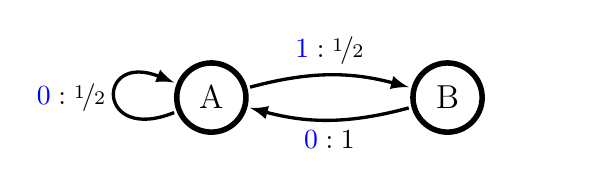
\begin{tikzpicture}[style=vaucanson,
                        bend angle=15,
                        scale=1,
                        every node/.style={transform shape}]
      \node [state] (A)              {A};
      \node [state] (B) [right of=A] {B};

      \path (A) edge [loop left] node {$\Edge{0}{\half}$} (A)
            (A) edge [bend left] node {$\Edge{1}{\half}$} (B)
            (B) edge [bend left] node {$\Edge{0}{1}$}     (A);
      \path (B) edge [loop right, draw=none] node {} (B);
    \end{tikzpicture}
    \label{subfig:golden_mean_process}
  } \\
  \subfloat[
      The anatomy of the Golden Mean process. Here, $\alpha =
      \frac{\log_2{3}}{2}$.
    ]{
    \begin{tikzpicture}
      \idiagramsetup

      \draw [ultra thick, pres_color] \present;
      \draw [ultra thick, past_color] \fcsz;
      \draw [ultra thick, futu_color] \rcso;
      \draw [ultra thick, black] \fcso;

      \labelpresent;
      \labelfcsz;
      \labelrcso;
      \labelfcso;

      \node at \locationa {0};
      \node at \locationb {{\footnotesize $\alpha - \nicefrac{1}{3}$}};
      \node at \locationc {0};
      \node at \locationd {{\footnotesize $1 - \alpha$}};
      \node at \locatione {{\footnotesize $3\alpha - \nicefrac{7}{3}$}};
      \node at \locationf {{\footnotesize $1 - \alpha$}};
      \node at \locationg {0};
      \node at \locationh {0};
      \node at \locationi {\nicefrac{2}{3}};
      \node at \locationj {\nicefrac{2}{3}};
    \end{tikzpicture}
    \label{subfig:golden_mean_anatomy}
  }
  \caption{The Golden Mean process.}
  \label{fig:golden_mean}
\end{figure}

\begin{figure}
  \centering
  \subfloat[The Even Process.]{
    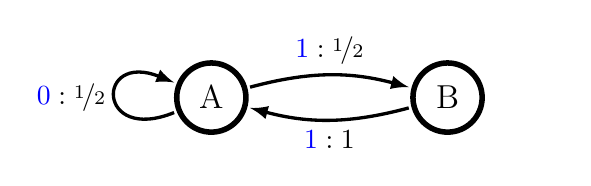
\begin{tikzpicture}[style=vaucanson,
                        bend angle=15,
                        scale=1,
                        every node/.style={transform shape}]
      \node [state] (A)              {A};
      \node [state] (B) [right of=A] {B};

      \path (A) edge [loop left] node {$\Edge{0}{\half}$} (A)
            (A) edge [bend left] node {$\Edge{1}{\half}$} (B)
            (B) edge [bend left] node {$\Edge{1}{1}$}     (A);
      \path (B) edge [loop right, draw=none] node {} (B);
    \end{tikzpicture}
    \label{subfig:even_process}
  } \\
  \subfloat[
      The anatomy of the Even process. Here, $\alpha = \frac{\log_2{3}}{2}$.
    ]{
    \begin{tikzpicture}
      \idiagramsetup

      \draw [ultra thick, pres_color] \present;
      \draw [ultra thick, past_color] \fcsz;
      \draw [ultra thick, futu_color] \rcso;
      \draw [ultra thick, black] \fcso;

      \labelpresent;
      \labelfcsz;
      \labelrcso;
      \labelfcso;

      \node at \locationa {0};
      \node at \locationb {0};
      \node at \locationc {\nicefrac{2}{3}};
      \node at \locationd {0};
      \node at \locatione {{\footnotesize $2\alpha - 2$}};
      \node at \locationf {\nicefrac{2}{3}};
      \node at \locationg {0};
      \node at \locationh {\nicefrac{2}{3}};
      \node at \locationi {0};
      \node at \locationj {0};
    \end{tikzpicture}
    \label{subfig:even_anatomy}
  }
  \caption{The Even process.}
  \label{fig:even}
\end{figure}

\begin{figure}
  \centering
  \subfloat[The (insert name here) Process.]{
    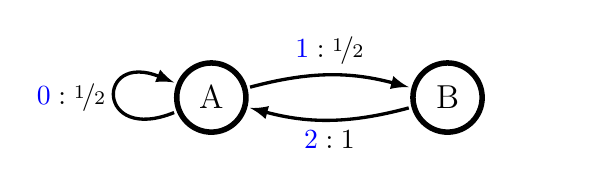
\begin{tikzpicture}[style=vaucanson,
                        bend angle=15,
                        scale=1,
                        every node/.style={transform shape}]
      \node [state] (A)              {A};
      \node [state] (B) [right of=A] {B};

      \path (A) edge [loop left] node {$\Edge{0}{\half}$} (A)
            (A) edge [bend left] node {$\Edge{1}{\half}$} (B)
            (B) edge [bend left] node {$\Edge{2}{1}$}     (A);
      \path (B) edge [loop right, draw=none] node {} (B);
    \end{tikzpicture}
    \label{subfig:noname_process}
  } \\
  \subfloat[
      The anatomy of the (insert name here) process. Here, $\alpha =
      \frac{\log_2{3}}{2}$.
    ]{
    \begin{tikzpicture}
      \idiagramsetup

      \draw [ultra thick, pres_color] \present;
      \draw [ultra thick, past_color] \fcsz;
      \draw [ultra thick, futu_color] \rcso;
      \draw [ultra thick, black] \fcso;

      \labelpresent;
      \labelfcsz;
      \labelrcso;
      \labelfcso;

      \node at \locationa {0};
      \node at \locationb {0};
      \node at \locationc {\nicefrac{2}{3}};
      \node at \locationd {0};
      \node at \locatione {{\footnotesize $2\alpha - \nicefrac{4}{3}$}};
      \node at \locationf {\nicefrac{2}{3}};
      \node at \locationg {0};
      \node at \locationh {0};
      \node at \locationi {0};
      \node at \locationj {0};
    \end{tikzpicture}
    \label{subfig:noname_anatomy}
  }
  \caption{The (insert name here) process.}
  \label{fig:noname}
\end{figure}

\bibliography{faoab}

\cleardoublepage

\appendix


\end{document}
